
\begin{figure}[!ht]
\centering
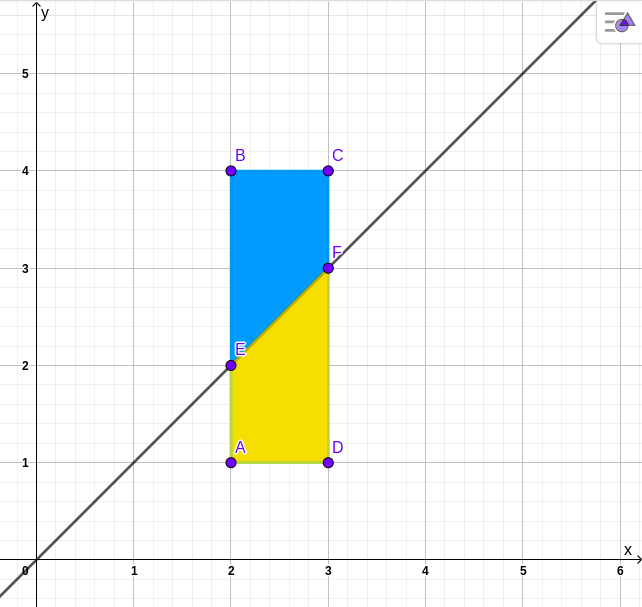
\includegraphics[width=\columnwidth]{solutions/in/2021/figures/figure.png}
\caption{Probability Distribution of (X, Y)}
\label{fig:Nuruhuhuhuhuhuhu}
\end{figure}

In figure \ref{fig:Nuruhuhuhuhuhuhu}, rectangle ABCD represents sample space of (X, Y). $Y \le X$ for any point (X, Y) if and only if the point lies on or below line EF. Therefore 
\begin{align}
    \pr{Y \le X} = \cfrac{Area\; of\; AEFD}{Area\; of\; ABCD}\\
                 = \cfrac{1}{2}    
\end{align}

Alternately, we have PDF and CDF of X and Y given by 
\begin{align}
    f_X(x) = 
    \begin{cases}
    1 & 2\le x\le 3\\
    0 & otherwise
    \end{cases}
\end{align}
\begin{align}
    F_X(x) = 
    \begin{cases}
    0   & x < 2\\
    x-2 & 2\le x\le 3\\
    1   & x > 3
    \end{cases}
\end{align}
\begin{align}
    f_Y(x) = 
    \begin{cases}
    1 & 1\le x\le 4\\
    0 & otherwise
    \end{cases}
\end{align}
\begin{align}
    F_Y(x) = 
    \begin{cases}
    0   & x < 1\\
    \cfrac{x-1}{3} & 1\le x\le 4\\
    1   & x > 4
    \end{cases}
\end{align}
Thus 
\begin{align}
    \pr{Y\le X} &= \int_{-\infty}^{\infty} F_Y(x)f_X(x)dx\\
                &= \int_2^3 \cfrac{x-1}{3}dx\\
                &= \cfrac{1}{2}
\end{align}


